\documentclass{article}
\usepackage[top=1cm, left=1.5cm, right=1.5cm, bottom=1.5cm]{geometry}
\usepackage{graphicx}
\usepackage{wrapfig}
\graphicspath{{./img/}}
\usepackage{amsmath}
\usepackage{tcolorbox}
\usepackage{tikz-cd}
\usepackage{amssymb}
\usepackage{apacite}
\bibliographystyle{apacite}
\setlength{\parindent}{0pt}
\setlength{\parskip}{1em} 
 
\title{Ecuaciones Vectoriales}
\author{Pablo Darío}
\date{14/12/2023}
 
\begin{document}
\maketitle

Importantes propiedades de sistemas lineales se pueden describir mediante el concepto y la notación de vectores. Por ahora, \textbf{vector} significará una lista ordenada de números. Esta idea sencilla permite realizar, de manera rápida, interesantes e importantes aplicaciones.

\section*{Vectores en $\mathbb{R}^2$}
 
Una matriz con una sola columna es un \textbf{vector columna} o simplemente un \textbf{vector}. Ejemplos:

\begin{equation*}
    u = \begin{bmatrix}
        3\\
        -1
    \end{bmatrix}
    , \quad v = \begin{bmatrix}
        .2\\
        .3
    \end{bmatrix}
    , \quad w = \begin{bmatrix}
        w1\\
        w2
    \end{bmatrix}
\end{equation*}

donde $w_1$ y $w_2$ son números reales. $\mathbb{R}^2$ denota el conjunto de todos los vectores con dos entradas. La $\mathbb{R}$ representa los números reales que aparecen como entradas en los vectores y el exponente $2$ indica que cada vector contiene dos entradas.

Dos vectores en $\mathbb{R}^2$ son \textbf{iguales} si y solo si sus entradas correspondientes son iguales. Así $\begin{bmatrix} 4\\7 \end{bmatrix}$ y $\begin{bmatrix} 7\\4 \end{bmatrix}$ no son iguales, porque los vectores en $\mathbb{R}^2$ son pares ordenados de números reales.

\subsection*{Propiedades}

\begin{large}
    \textbf{Suma de Vectores}
\end{large}

Dados dos vectores $u$ y $v$ en $\mathbb{R}^2$, su \textbf{suma} es el vector $u + v$, que se obtiene al sumar las entradas correspondientes de $u$ y $v$. Ejemplo:

\begin{equation*}
    \begin{bmatrix}
        1\\
        -2
    \end{bmatrix}
    + \begin{bmatrix}
        2\\
        5
    \end{bmatrix}
    = \begin{bmatrix}
        1 + 2 \\
        -2 + 5
    \end{bmatrix}
    = \begin{bmatrix}
        3 \\
        3
    \end{bmatrix}
\end{equation*}

\begin{large}
    \textbf{Multiplicación por un Escalar}
\end{large}

Considerando un vector \textbf{u} y un número real $c$, el múltipli escalar de \textbf{u} por $c$ es el vector $c$\textbf{u}, que se obtiene al multiplicar por $c$ cada entrada en \textbf{u}. Ejemplo:

\begin{equation*}
    \text{si} \quad u = \begin{bmatrix}
        3\\
        -1
    \end{bmatrix} 
    \quad \text{y} \quad c = 5, \quad \text{entonces} \quad
    c \textbf{u} = 5 \begin{bmatrix}
        3\\
        -1
    \end{bmatrix}
    = \begin{bmatrix}
        3 \times 5 \\
        -1 \times 5
    \end{bmatrix}
    = \begin{bmatrix}
        15 \\
        -5
    \end{bmatrix}
\end{equation*}

El número $c$ en $c$\textbf{u} se llama escalar; se escribe en cursivas, para así distinguirlo del vector \textbf{u}.

Es posible combinar las operaciones de multiplicación por un escalar y suma vectorial, como en el siguiente ejemplo:

\pagebreak

\begin{large}
    \textbf{Ejemplo}
\end{large}

A partir de \textbf{u} = $\begin{bmatrix} 1\\-2 \end{bmatrix}$ y \textbf{v} = $\begin{bmatrix} 2\\-5 \end{bmatrix}$, encuentre 4\textbf{u}, (-3)\textbf{v} y $4\textbf{u} + (-3)\textbf{v}$.

\begin{equation*}
    4u = \begin{bmatrix}
        4\\
        -8
    \end{bmatrix} 
    ,\quad 
    -3v = \begin{bmatrix}
        -6\\
        15
    \end{bmatrix}
\end{equation*}

Por lo tanto

\begin{equation*}
    4u + (-3v) = \begin{bmatrix}
        4\\
        -8
    \end{bmatrix} 
    ,\quad 
    + \begin{bmatrix}
        -6\\
        15
    \end{bmatrix}
    = \begin{bmatrix}
        -2\\
        7
    \end{bmatrix}
\end{equation*}

Un vector también se puede representar con paréntesis, por ejemplo el vector columna $\begin{bmatrix} 3\\-1 \end{bmatrix}$ se puede representar como $\begin{pmatrix} 3, -1 \end{pmatrix}$. En este caso los paréntesis y la coma distinguen al vector (3, -1) de la matriz $\begin{bmatrix} 3 & -1 \end{bmatrix}$ que se representa con corchetes y sin coma. Así bien: 

\begin{equation*}
    \begin{bmatrix}
        3\\
        -1
    \end{bmatrix} 
    \neq 
    \begin{bmatrix}
        3 & -1
    \end{bmatrix}
\end{equation*}

Ya que las matrices tienen distintas formas, aunque las entradas sean iguales.

\subsection*{Geometría en $\mathbb{R}^2$}

Cada punto en el plano está determinado por un par ordenado de puntos, así bien, es posible identificar un punto geométrico $(a, b)$ con el vector columna  $\begin{bmatrix} a\\b \end{bmatrix}$. Así, puede considerarse a $\mathbb{R}^2$ como el conjunto de todos los puntos del plano.

\begin{figure}[ht]
    \centerline{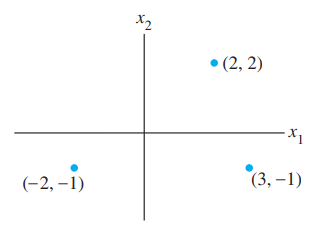
\includegraphics[width=0.3\textwidth]{image6.png}}
    \caption{Vectores como puntos}
    \label{}
\end{figure}

\begin{tcolorbox}[colback=green!20!white,colframe=green!80!black,title=Regla del Paralelogramo para la adición]
    Si \textbf{u} y \textbf{v} en $\mathbb{R}^2$ se representan como puntos en el plano, entonces \textbf{u} + \textbf{v} corresponde a un cuarto vértice del paralelogramo cuyos otros vértices son \textbf{u, 0} y \textbf{v}
\end{tcolorbox}

\begin{figure}[ht]
    \centerline{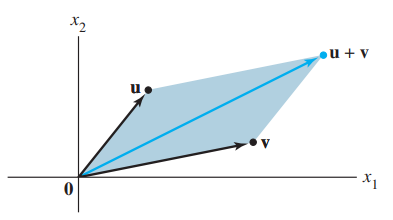
\includegraphics[width=0.3\textwidth]{image7.png}}
    \caption{Regla del paralelogramo}
    \label{}
\end{figure}

\begin{large}
    \textbf{Ejemplo}
\end{large}

Los vectores \textbf{u} = $\begin{bmatrix} 2\\2 \end{bmatrix}$, \textbf{v} = $\begin{bmatrix} -6\\1 \end{bmatrix}$ y \textbf{u + v} = $\begin{bmatrix} -4\\3 \end{bmatrix}$ forman el siguiente paralelogramo:

\begin{figure}[ht]
    \centerline{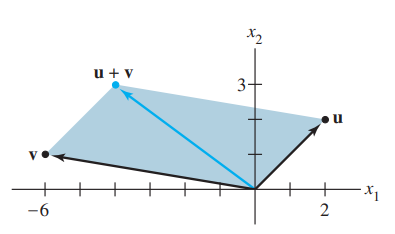
\includegraphics[width=0.3\textwidth]{image8.png}}
    \caption{Ejemplo Paralelogramo}
    \label{}
\end{figure}

El conjunto de todos los múltiplos escalares de un vector diferente de cero o no nulo, fijo, es una recta que pasa por el origen, (0, 0)

Sea \textbf{u} = $\begin{bmatrix} 3\\-1 \end{bmatrix}$. Representa en el plano \textbf{u}, 2 \textbf{u} y -$\frac{2}{3}$ \textbf{u}.

Así bien, \textbf{u} = $\begin{bmatrix} 3\\-1 \end{bmatrix}$, 2\textbf{u} = $\begin{bmatrix} 6\\-2 \end{bmatrix}$ y $\frac{2}{3}$ \textbf{u} = $\begin{bmatrix} -2\\ \frac{2}{3} \end{bmatrix}$. La flecha para 2\textbf{u} es el doble del largo que la flecha para \textbf{u} y va en el mismo sentido que \textbf{u}. La flecha para - $\frac{2}{3}$\textbf{u} es dos tercios de la longitud de la flecha para \textbf{u} y va en sentido opuesto. En general, la longitud de la flecha para $c\textbf{u}$ es $|c|$ veces la longitud de la flecha para \textbf{u}. 

\begin{figure}[ht]
    \centerline{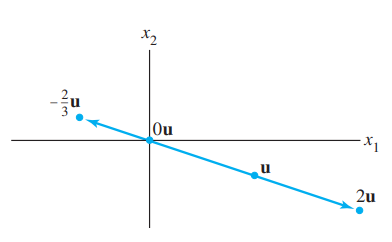
\includegraphics[width=0.3\textwidth]{image9.png}}
    \caption{Múltiplos del vector u}
    \label{}
\end{figure}

\subsection*{Vectores en $\mathbb{R}^n$}

Los vectores en $\mathbb{R}^3$ son matrices columna de $3 \times 1$ con tres entradas. Se representan geométricamente mediante puntos en un espacio coordenado tridimensional; algunas veces se incluyen flechas desde el origen para dar una mayor claridad visual.

Si $n$ es un entero positivo, $\mathbb{R}^n$ denota la colección de todas las listas de $n$ números reales, generalmente escritas como matrices columna de $n \times 1$ del tipo $$\begin{bmatrix} u_1\\u_2\\ \vdots\\u_n \end{bmatrix}$$

El vector cuyas entradas son todas cero se llama \textbf{vector cero} y se denota con 0. La igualdad de vectores en $\mathbb{R}^n$ y las operaciones de multiplicación escalar y suma vectorial en $\mathbb{R}^n$ se definen entrada por entrada como en $\mathbb{R}^2$

\begin{tcolorbox}[colback=blue!10!white,colframe=blue!60!black,title=Propiedades Algebraicas de $\mathbb{R}^n$]
    Para todo \textbf{u, v, w} en $\mathbb{R}^n$ y para todos los escalares $c$ y $d$:
    \begin{itemize}
        \item[1.-] \textbf{u} + \textbf{v} = \textbf{v} + \textbf{u} \hspace{65mm} 5.- $c$(\textbf{u} + \textbf{v}) = $c$\textbf{u} + $c$\textbf{v}
        \item[2.-] (\textbf{u} + \textbf{v}) + \textbf{w} = \textbf{u} + (\textbf{v} + \textbf{w}) \hspace{43.5mm} 6.- ($c$ + $d$)\textbf{u} = $c$\textbf{u} + $d$\textbf{u}
        \item[3.-] \textbf{u} + 0 = \textbf{u} \hspace{73mm} 7.- $c$($d$\textbf{u}) = ($cd$)(\textbf{u})
        \item[4.-] \textbf{u} + (-\textbf{u}) = -\textbf{u} + \textbf{u} = 0 \hspace{53.2mm} 8.-1\textbf{u} = \textbf{u}    
    \end{itemize}
\end{tcolorbox}

\subsection*{Combinaciones Lineales}

Dados los vectores $v_1,v_2,\dots, v_p$ en $\mathbb{R}^n$ y dados los escalares $c_1,c_2,\dots, c_p$ el vector definido $\mathbf{y}$ definido por:$$\mathbf{y} = c_1v_1 + \dotsb +  c_pv_p$$ se llama \textbf{combinaciòn lineal} de $v_1, \dotsb, v_p$ con pesos $c_1, \dotsb, c_p$. Los pesos en una combinación lineal pueden ser cualesquiera números reales, incluyendo el cero, algunos ejemplos de combinaciones lineales de $v_1$ y $v_2$ son $$\sqrt{3}v_1 + v_2, \quad \frac{1}{2}v_1(= \frac{1}{2}v_1 + 0v_2), \quad 0 (= 0v_1 + 0v_2)$$

\begin{figure}[ht]
    \centerline{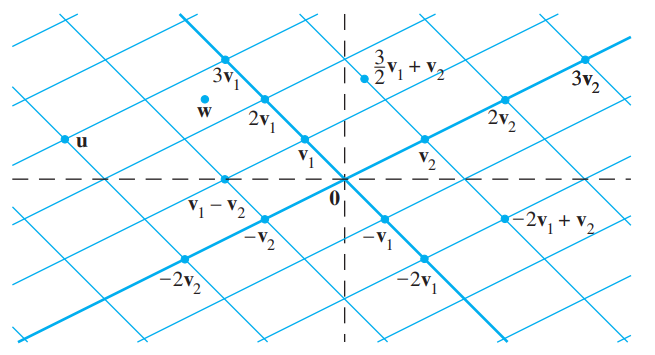
\includegraphics[width=0.3\textwidth]{image10.png}}
    \caption{Combinaciones Lineales}
    \label{}
\end{figure}

\begin{large}
    \textbf{Ejemplo}
\end{large}

Sean \textbf{$v_1$} = $\begin{bmatrix} 1\\-2\\-5 \end{bmatrix}$, \textbf{$v_2$} = $\begin{bmatrix} 2\\5\\6 \end{bmatrix}$  y \textbf{$b$} = $\begin{bmatrix} 7\\4\\-3 \end{bmatrix}$. Determine si \textbf{$b$} se puede generar como una combinación lineal de \textbf{$v_1$} y \textbf{$v_2$}. Es decir, determine si existen pesos $x_1$ y $x_2$ tales que $$x_1\textbf{$v_1$} + x_2\textbf{$v_2$} = \textbf{$b$}$$

Así bien, gracias a las propiedades de multiplicación por un escalar y suma vectorial, podemos reescribir la ecuación como:

\begin{equation*}
    x_1 \begin{bmatrix}
        1\\-2\\-5
    \end{bmatrix} 
    +x_2 \begin{bmatrix}
        2\\5\\6
    \end{bmatrix}
    = \begin{bmatrix}
        7\\4\\-3
    \end{bmatrix}
\end{equation*}

Aplicando las operaciones obtenemos

\begin{equation*}
    \begin{bmatrix}
        x_1\\-2x_1\\-5x_1
    \end{bmatrix} 
    +\begin{bmatrix}
        2x_2\\5x_2\\6x_2
    \end{bmatrix}
    = \begin{bmatrix}
        7\\4\\-3
    \end{bmatrix}
\end{equation*}

y 

\begin{equation*}
    \begin{bmatrix}
        x_1 + 2x_2\\-2x_1 + 5x_2 \\-5x_1 + 6x_2
    \end{bmatrix} 
    = \begin{bmatrix}
        7\\4\\-3
    \end{bmatrix}
\end{equation*}

Los vectores en los miembros izquierdo y derecho de son iguales si y solo si sus entradas correspondientes son iguales. Es decir, $x_1$ y $x_2$ hacen válida la ecuación vectorial $x_1\textbf{$v_1$} + x_2\textbf{$v_2$} = \textbf{$b$}$ si y solo si $x_1$ y $x_2$ satisfacen el siguiente sistema:

\begin{equation*}
    \begin{array}{ccc}
        x_1 &+ 2x_2 &= 7\\
        -2x_1 &+ 5x_2 &= 4\\
        -5x_1 &+ 6x_2 &= -3
    \end{array}
\end{equation*}

Ahora tenemos que resolver el sistma para ver si existen valores para $x_1$ y $x_2$ que hagan válido el sistema; para ello reducimos por filas la matriz aumentada como sigue:

\begin{equation}
    \left[\begin{array}{rr|r}
    1 & 2 & 7 \\
    -2 & 5 & 4 \\
    -5 & 6 & -3
    \end{array}\right] \sim\left[\begin{array}{rr|r}
    1 & 2 & 7 \\
    0 & 9 & 18 \\
    0 & 16 & 32
    \end{array}\right] \sim\left[\begin{array}{rr|r}
    1 & 2 & 7 \\
    0 & 1 & 2 \\
    0 & 16 & 32
    \end{array}\right] \sim\left[\begin{array}{ll|l}
    1 & 0 & 3 \\
    0 & 1 & 2 \\
    0 & 0 & 0
    \end{array}\right]
\end{equation}

Así obtenemos que la solución es $x_1 = 3$ y $x_2 = 2$. Así que \textbf{b} es una combinación lineal de \textbf{$v_1$} y \textbf{$v_2$}. Esto es, 

\begin{equation*}
    3 \begin{bmatrix}
        1\\-2\\-5
    \end{bmatrix} 
    +2 \begin{bmatrix}
        2\\5\\6
    \end{bmatrix}
    = \begin{bmatrix}
        7\\4\\-3
    \end{bmatrix}
\end{equation*}

Por brevedad se puede escribir la matriz aumentada en una forma que identifique sus columnas fácilemnte como $\begin{bmatrix} \textbf{$v_1$} & \textbf{$v_2$} & b \end{bmatrix}$

\begin{tcolorbox}[colback=green!20!white,colframe=green!80!black,title=Ecuación Vectorial y Sistema lineal]
    Una ecuación vectorial $$x_1\textbf{$v_1$} + x_2\textbf{$v_2$} + \dotsb + x_n\textbf{$v_n$} = \textbf{$b$}$$ tiene el mismo conjunto solución que el sistema lineal cuya matriz aumentada es $$\begin{bmatrix} \textbf{$v_1$} & \textbf{$v_2$} \dotsb & \textbf{$v_n$} & b \end{bmatrix}$$

    En particular. \textbf{b} se puede generar por una combinación lineal de $v_1, v_2,\dots, v_n$ si y solo si existe una solución al sistema lineal correspondiente a la matriz aumentada anterior.
\end{tcolorbox}

\begin{tcolorbox}[colback=blue!10!white,colframe=blue!60!black,title=Conjunto de Combinaciones Lineales]
    Si $v_1,v_2,\dots, v_p$ están en $\mathbb{R}^n$, entonces el conjunto de todas las combinaciones lineales de $v_1,v_2,\dots, v_p$ se donta como Gen\{$v_1,v_2,\dots, v_p$\} y se llama \textbf{subconjunto de $\mathbb{R}^n$ extendido o generado por $v_1,v_2,\dots, v_p$}. Es decir Gen\{$v_1,v_2,\dots, v_p$\} es el conjunto de todos los vectores que se pueden escribir en la forma $$c_1v_1 + c_2v_2 + \dots + c_pv_p$$
    con escalares $c_1,c_2,\dots, c_p$
\end{tcolorbox}

Preguntar si un vector \textbf{b} está en Gen\{$v_1,v_2,\dots, v_p$\} equivale a preguntar si la ecuación vectorial $$x_1v_1 + x_2v_2 + \dots + x_pv_p$$ tiene una solución. La cual se puede reescribir como, 

\begin{equation*}
    x_1 \begin{bmatrix} v_1 \end{bmatrix} 
    +x_2 \begin{bmatrix} v_2 \end{bmatrix}
    + \dotsb + x_p \begin{bmatrix} v_p \end{bmatrix}
    = \begin{bmatrix} b \end{bmatrix}
\end{equation*}

o de manera equivalente, si el sistema lineal con la matriz aumentada $\begin{bmatrix} v_1 & v_2 & \dotsb & v_p & b \end{bmatrix}$ tiene una solución.

Observe que Gen\{$v_1,v_2,\dots, v_p$\} contiene a cada múltiplo escalar de $v_1$ (por ejemplo), ya que $cv_1 = cv_1 + 0v_2 + \dotsb + 0v_p$. En particular, el vector cero debe estar en Gen\{$v_1,v_2,\dots, v_p$\}.

\subsection*{Descripción Geométrica de Gen\{v\} y de Gen\{u, v\}}

Sea v un vector diferente de cero en $\mathbb{R}^3$. Entonces Gen\{\textbf{$v$}\} es el conjunto de todos los múltiplos escalares de \textbf{$v$}, que es el conjunto de puntos sobre la recta en en $\mathbb{R}^3$ que pasa por \textbf{$v$} y 0. 

Si \textbf{$u$} y \textbf{$v$} son vectores diferentes de cero en $\mathbb{R}^3$, y \textbf{$v$} no es un múltiplo de \textbf{$u$}, entonces Gen\{\textbf{$u$}, \textbf{$v$}\} es el plano en $\mathbb{R}^3$ que contiene a \textbf{$u$}, \textbf{$v$} y 0. En particular, Gen\{\textbf{$u$}, \textbf{$v$}\} contiene la recta en $\mathbb{R}^3$ que pasa por \textbf{$u$} y 0, y la recta que pasa por \textbf{$v$} y 0.

\begin{figure}[ht]
    \centerline{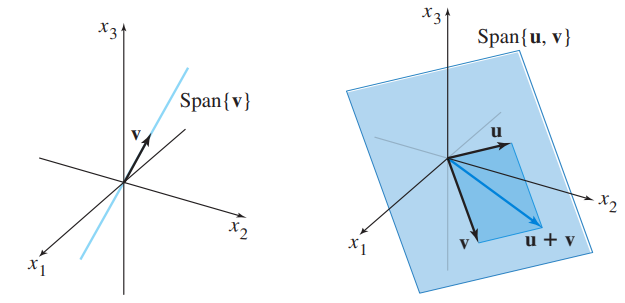
\includegraphics[width=0.6\textwidth]{image11.png}}
    \caption{Gen\{\textbf{$u$}\} y Gen\{\textbf{$u$}, \textbf{$v$}\}}
    \label{}
\end{figure}

\begin{large}
    \textbf{Ejemplo}
\end{large}

Sean \textbf{$a_1$} = $\begin{bmatrix} 1\\-2\\3 \end{bmatrix}$, \textbf{$a_2$} = $\begin{bmatrix} 5\\-13\\-3 \end{bmatrix}$ y \textbf{$b$} = $\begin{bmatrix} -3\\8\\1 \end{bmatrix}$. Entonces  Gen\{\textbf{$a_1$}, \textbf{$a_2$}\} es un plano que pasa por el origen en $\mathbb{R}^3$. ¿Está \textbf{b} en ese plano?

Para responder esto debemos ver si \textbf{$b$} es una combinación lineal de \textbf{$a_1$} y \textbf{$a_2$}; es decir ¿Tiene solución la ecuación $x_1$\textbf{$a_1$} + $x_2$\textbf{$a_2$} = \textbf{$b$}? Así bein debemos reducir por la filas la ,atriz aumentada $\begin{bmatrix} a_1 & a_2 & a_3 \end{bmatrix}$

\begin{equation*}
    \left[\begin{array}{rrr}
    1 & 5 & -3 \\
    -2 & -13 & 8 \\
    3 & -3 & 1
    \end{array}\right] \sim\left[\begin{array}{rrr}
    1 & 5 & -3 \\
    0 & -3 & 2 \\
    0 & -18 & 10
    \end{array}\right] \sim\left[\begin{array}{rrr}
    1 & 5 & -3 \\
    0 & -3 & 2 \\
    0 & 0 & -2
    \end{array}\right]
\end{equation*}

Por lo tanto, vemos que el sistema es inconsistente, debido a que la tercera ecuación es  0 = -2. La ecuación vectorial $x_1$\textbf{$a_1$} + $x_2$\textbf{$a_2$} = \textbf{$b$} no tiene solución, de manera que \textbf{$b$} no está en Gen\{\textbf{$a_1$}, \textbf{$a_2$}\}.\cite{DavidC}

\pagebreak
\bibliography{Referencias}
\end{document}